\documentclass{standalone}
\usepackage{tikz}

\begin{document}
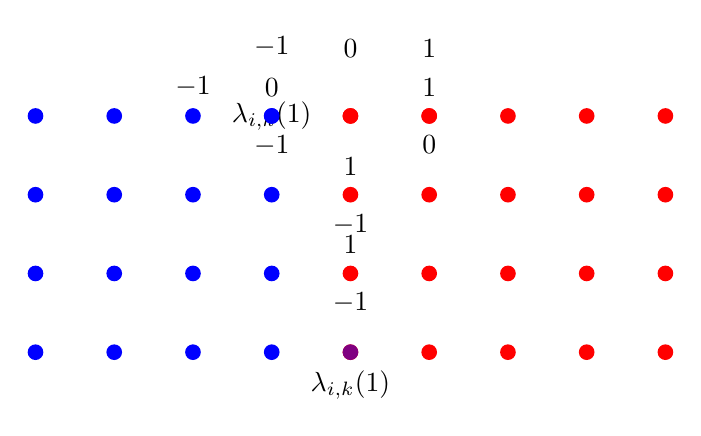
\begin{tikzpicture}
    % Draw the points
    \foreach \y in {0,...,3} {
        \foreach \x in {-4,...,4} {
            \ifnum\x<0
                \node at (\x, \y) [circle, fill=blue, inner sep=2pt] {};
            \else
                \node at (\x, \y) [circle, fill=red, inner sep=2pt] {};
            \fi
        }
    }

    % Draw the labels
    \node at (0, 0) [circle, fill=violet, inner sep=2pt, label=below:{\(\lambda_{i,k}(1)\)}] {};
    \node at (0, 1) [label=below:{\(-1\)}, label=above:{\(1\)}] {};
    \node at (0, 2) [label=below:{\(-1\)}, label=above:{\(1\)}] {};
    \node at (-1, 3) [label=below:{\(-1\)}, label=above:{\(0\)}, label=center:{\(\lambda_{i,k}(1)\)}] {}; % Placed at the center of the point
    \node at (1, 3) [label=below:{\(0\)}, label=above:{\(1\)}] {};

    % Adjust -1 and 0 labels on the top row for clarity
    \node at (-1, 3) [circle, fill=blue, inner sep=2pt] {};
    \node at (0, 3) [circle, fill=red, inner sep=2pt] {};
    \node at (1, 3) [circle, fill=red, inner sep=2pt] {};

    % Additional labels for the top row points
    \node at (-2, 3) [label=above:{\(-1\)}] {};
    \node at (-1, 3.5) [label=above:{\(-1\)}] {}; % Adjusted to place above the point
    \node at (0, 3.5) [label=above:{\(0\)}] {};
    \node at (1, 3.5) [label=above:{\(1\)}] {};
\end{tikzpicture}
\end{document}